\begin{frame}{Une vie en Provence}
  \small
  Pour chaque blanc, quelle est la bonne conjugaison pour le verbe \emph{au passé composé}?
  \begin{columns}[t]
    \scriptsize
    \column{0.5\textwidth}
      \begin{enumerate}
        \item Ma grand-mère \underline{\uncover<2->{est née}} (naître) en Provence.
        \item Toute sa vie, elle \underline{\uncover<3->{a habité}} (habiter) dans cette région.
        \item Elle \underline{\uncover<4->{est morte}} (mourir) à 97 ans.
        \item Elle \underline{\uncover<5->{est devenue}} (devenir) si âgée
        \item parce qu'elle \underline{\uncover<6->{n'a jamais intervenu}} (ne jamais intervenir) dans les disputes du village.
      \end{enumerate}
      \vspace{0.2cm}
      \begin{flushright}
      Abbaye Notre-Dame de Sénaque \\
      à Gordes
      \end{flushright}
    \column{0.5\textwidth}
      \begin{enumerate}
        \setcounter{enumi}{5}
        \item Elle \underline{\uncover<7->{a toujours aidé}} (toujours aider) ses voisins.
        \item Elle \underline{\uncover<8->{a toujours lu}} (lire) les journaux,
        \item et elle \underline{\uncover<9->{a suivi}} (suivre) la politique.
        \item Elle \underline{\uncover<10->{a connu}} (connaître) deux guerres,
        \item parce qu'elle \underline{\uncover<11->{a vécu}} (vivre) longtemps.
      \end{enumerate}
      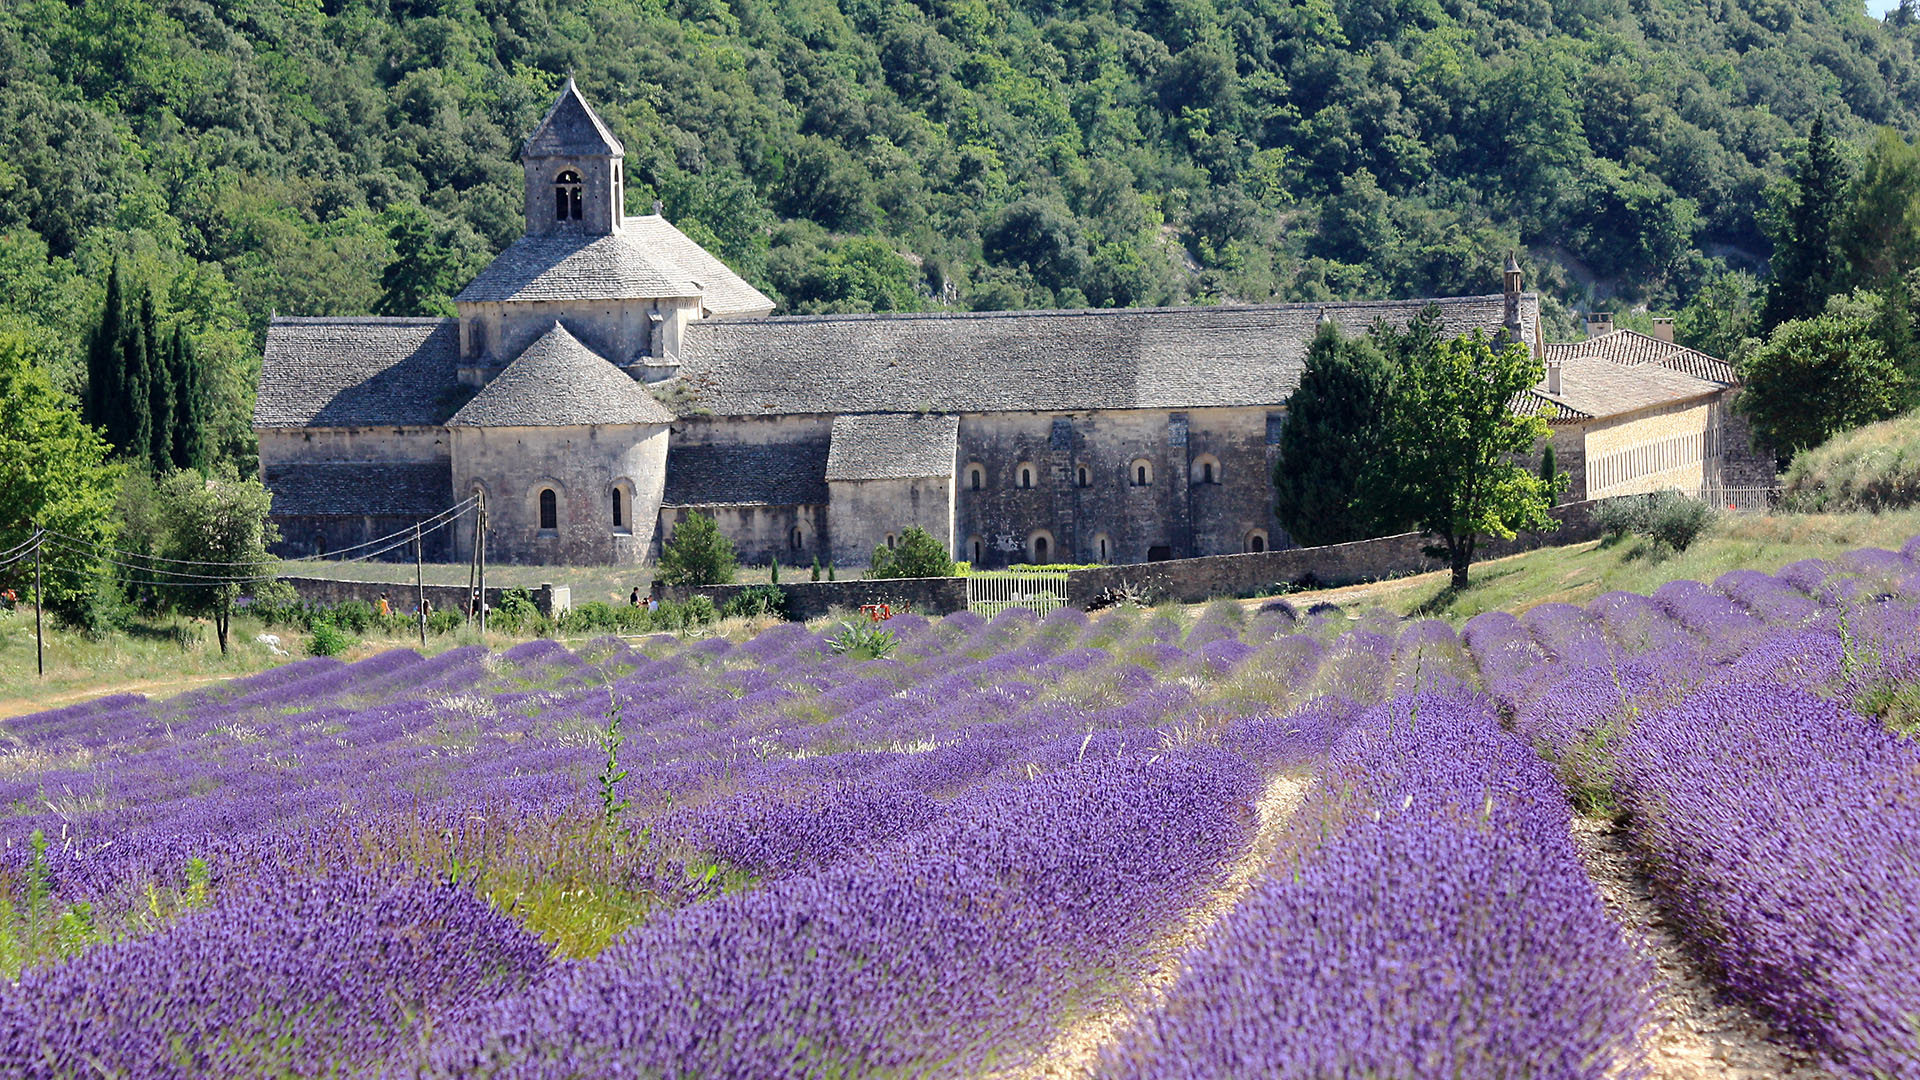
\includegraphics[scale=0.18]{abbaye.jpg}
  \end{columns}
\end{frame}